\documentclass{article}
\usepackage{authblk}
\usepackage{graphicx}
\usepackage{amsmath}

\usepackage[left=2.5cm,top=3cm,right=2.5cm,bottom=3cm,bindingoffset=0.5cm]{geometry}
\title{Using NPA data for sputtering estimations}
\author[1,2]{A. Adriaens}
\affil[1]{Laboratory for Plasma Physics LPP-ERM/KMS, Brussels, Belgium}
\affil[2]{Department of Applied Physics, Ghent University, Belgium}
\date{}

\setcounter{Maxaffil}{0}
\renewcommand\Affilfont{\itshape\small}

\begin{document}
\maketitle

\noindent
\begin{figure}[ht]
    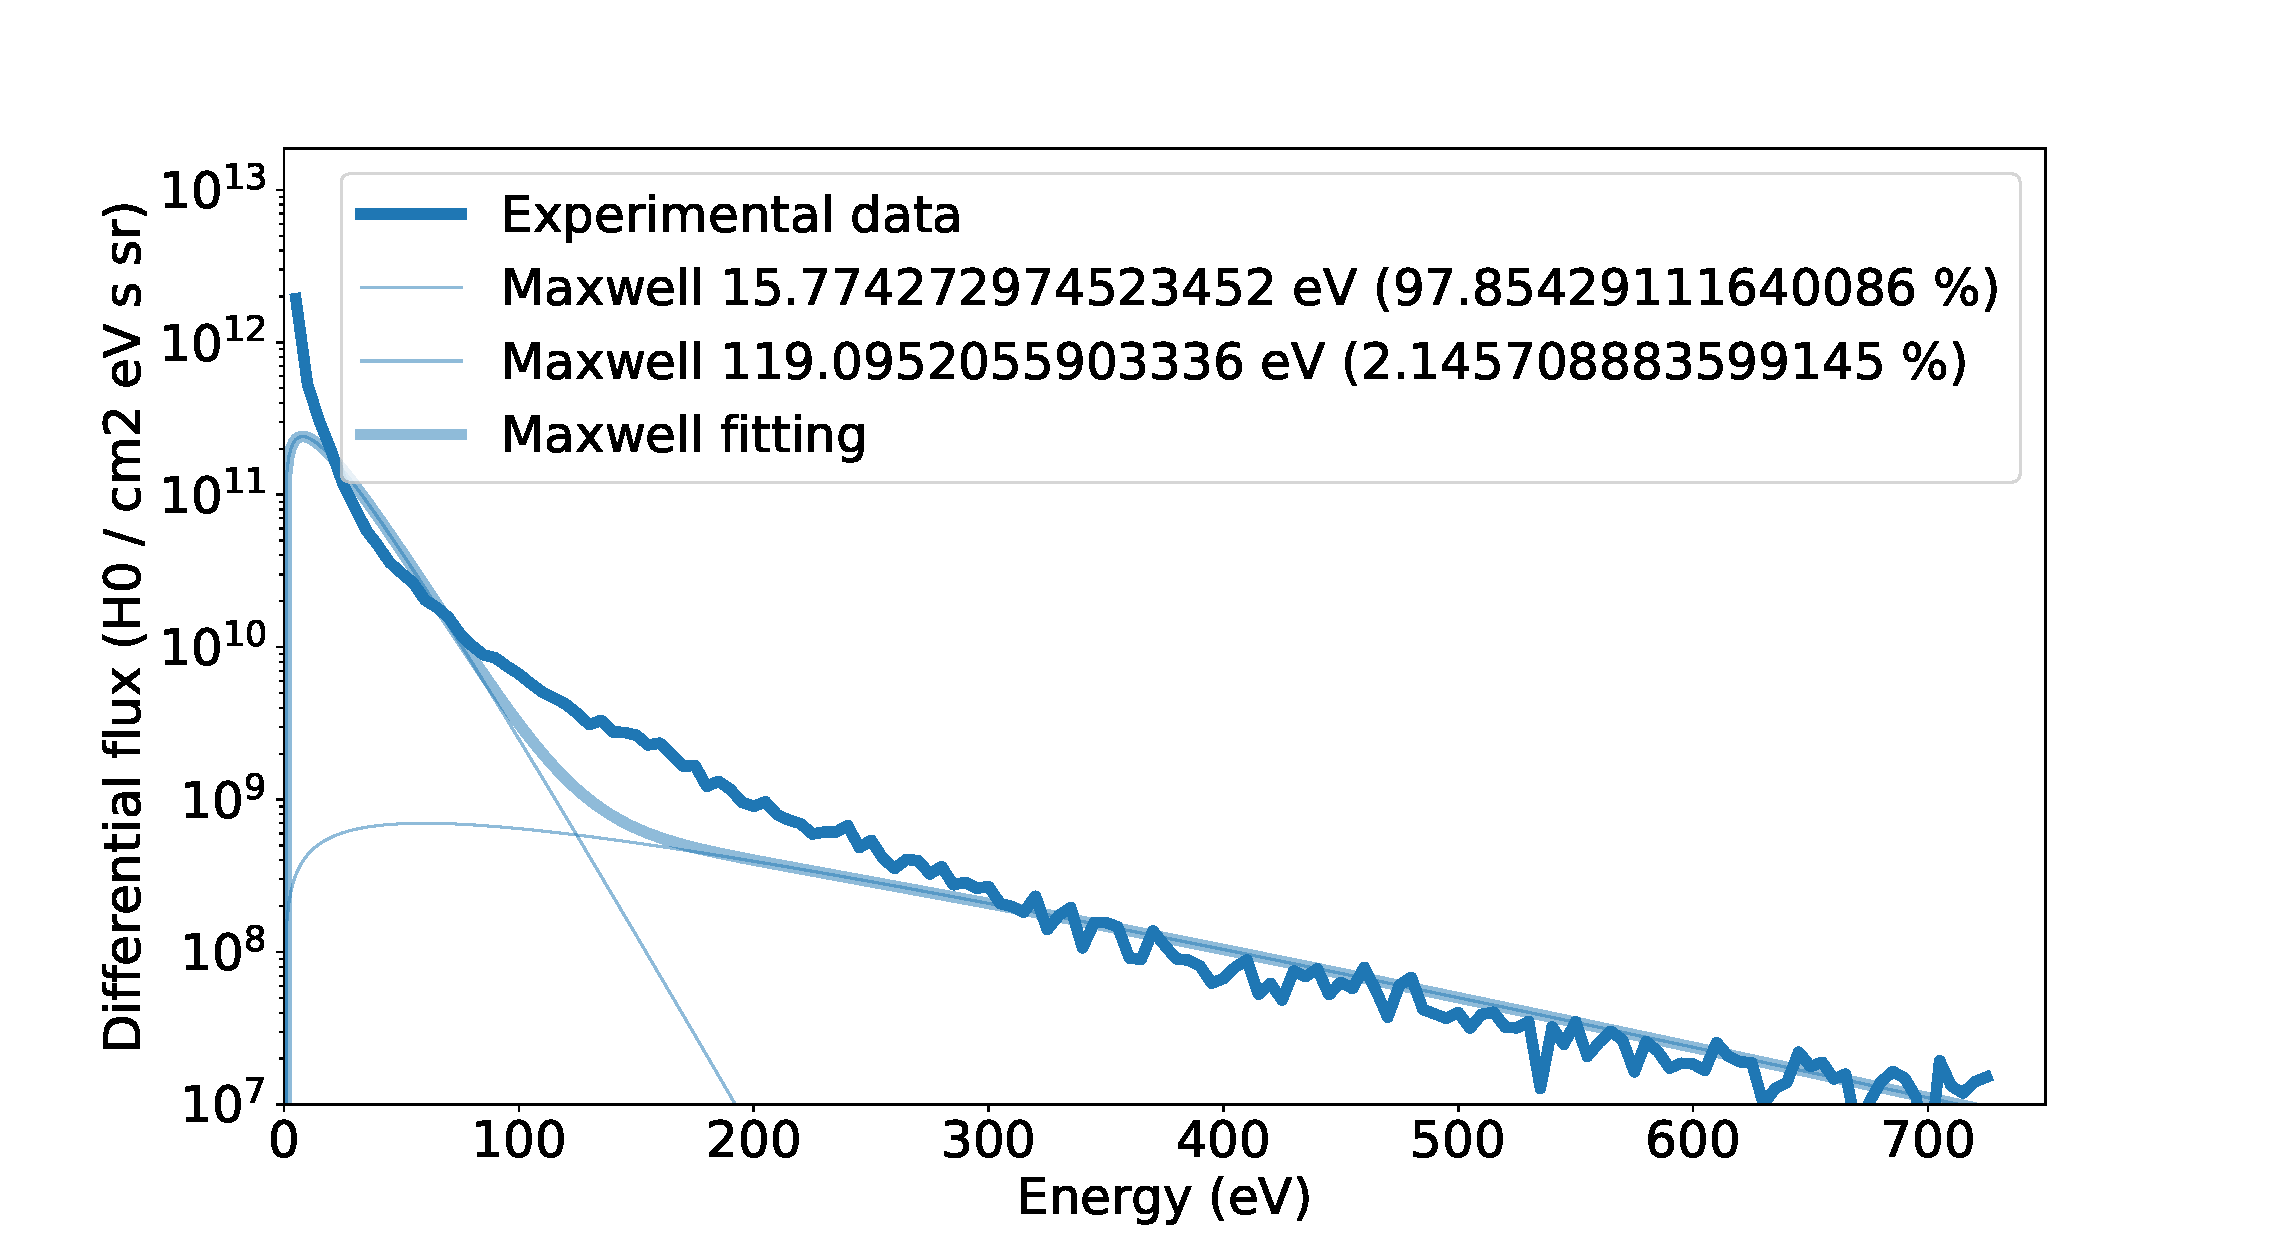
\includegraphics[width=\textwidth]{figures/NPA_example.pdf}
    \caption{The differential flux is easy to transform into a quantity we want by multiplying it with certain system parameters}
    \label{fig:examplemeasurement}
\end{figure}\\
The erosion rate due to the neutrals can be estimated from a NPA
measurement (an example of which is shown in figure
\ref{fig:examplemeasurement}) using the following formula:
\begin{equation}
    S = \frac{2\pi}{N} \int_E Y(E)\mathcal{F} (E) \text{dE}
    \label{eqn:ErosionRateFormal}
\end{equation}
With $Y(E)$ the yield of the gas on the material, $\mathcal{F}(E)$ the 
experimental differential flux and N the number density.
This is quite straightforward to see as:
\begin{itemize}
    \item The NPA covers a certain solid angle, this has been accounted for as
        can be seen in the unit of the example experiment (/sr meaning per
        steradian), we can get an approximation for the average
        flux in the vessel by assuming homogeneity and thus multiplying this
data by $2\pi$ steradians. 
    \item The differential flux in an energy bin causes sputtering, to get this
        sputtering rate we multiply by the yield $Y$ as it's defined to be the
        outgoing atoms per incoming, we integrate over all energies to get the
        full contribution. 
    \item The number density of the target $N$ dictates how the amount of
        outgoing atoms relates to the decrease in thickness.
\end{itemize}
In the software we use equation \ref{eqn:ErosionRateFormal} in the finite form,
summing over the energy bins:
\begin{equation}
S = \frac{2\pi}{N}\sum_{E_0}^{E_{\text{max}}} Y(E)\mathcal{F}(E)\Delta\text{E}
    \label{eqn:ErosionRateFinite}
\end{equation}
Where we may get the yield $Y(E)$ using the software RustBCA\cite{RustBCA} with
parameters from Wolfgang Eckstein's book \cite{eckstein2013computer}, assuming
perpendicular impingement.
%----------------------------------------------------------------------------------------
%	REFERENCE LIST
%----------------------------------------------------------------------------------------
\bibliographystyle{iopart-num}
\bibliography{Bibliography/sources}
%----------------------------------------------------------------------------------------

\end{document}
